
Se tienen $k$ vectores ordenados (de menor a mayor), cada uno con $n$ elementos, y queremos combinarlos en un \'unico vector ordenado (con $kn$ elementos). 
Una posible alternativa consiste en, utilizando un algoritmo cl\'asico, mezclar los dos primeros vectores, posteriormente mezclar el resultado con el tercero, y as\'i sucesivamente.

\begin{itemize}
    \item ¿Cu\'al ser\'ia el tiempo de ejecuci\'on de este algoritmo?
	\item Diseñe, analice la eficiencia e implemente un algoritmo de mezcla m\'as eficiente, 		  basado en \"divide y vencer\'as\".
	\item Realizar tambi\'en un estudio emp\'irico e h\'ibrido de la eficiencia de ambos 				  algoritmos.
\end{itemize}

\subsection{Estudio preliminar}
Plante\'ando el problema es posible imponer una cota superior te\'orica a la mezcla. Teniendo en cuenta que hay $kn$ elementos, si aplic\'asemos un algoritmo con eficiencia  $O(n)=nlog(n)$ deducimos que podemos encontrar un algoritmo de ordenaci\'on b\'asica con eficiencia $O(k,n)=nklog(nk)$. En este caso estar\'iamos representando los $k$ vectores de $n$ elementos como un \'unico vector, sin aprovechar a\'un el hecho de que partes del \"\ vector\ \" est\'an ordenadas.

Para obtener los datos, las gr\'aficas y los ajustes hemos usado un script 
Obligatorio/Script/script.sh, que compila y ejecuta los programas usados, ubicados en la carpeta Obligatorio/src/ y los scripts de gnuplot.

\subsubsection{Eficiencia te\'orica fuerza bruta}
El algoritmo propuesto consideramos que hace demasiadas escrituras en memoria.
Para la versi\'on a fuerza bruta en cada paso elegimos el m\'inimo de los primeros elementos de los $k$ vectores y lo ponemos en primer lugar, ser\'a el primer elemento del vector creciente resultante. Para el siguiente paso descartamos ese elemento y calculamos otra vez el m\'inimo, lo insertamos al final del vector resultante y as\'i sucesivamente.

Realmente la forma que usamos para descartar los elementos que vamos insertando es un vector de $k$ elementos que almacena los \'indices de cada vector. Inicialmente el \'indice de un vector es $0$, si usamos ese elemento el \'indice aumentar	\'a a $1$, para que no se repita, hasta recorrer todos los \'indices del i-\'esimo vector, $i \in [0,k-1]\cap \mathbb{N}$.

Buscar el m\'inimo en cada iteraci\'on es $O(k)=k$ ya que el vector de \'indices tiene $k$ elementos. El c\'alculo lo tenemos que hacer para cada elemento, hay $k$ vectores de $n$ elementos cada uno, por tanto se repetir\'a $kn$ veces.
\[\sum_{i=1}^{kn}k = nk^2 \implies \ O(k,n)=nk^2\]
		
\subsubsection{Eficiencia te\'orica divide y vencer\'as}
Para la versi\'on con divide y vencer\'as hemos usado una ver	si\'on del mergesort, pero con los primeros mont\'iculos ya creados, por tanto ser\'a mucho m\'as r\'apido que para $kn$ datos arbitrarios. 

El primer paso es pasar los vectores a un \'unico vector, con $O(k,n)=kn$

Posteriormente creamos las particiones para aprovechar el hecho de que hay partes del vector que ya est\'an ordenadas. En ese proceso lo que haremos es ir diviendo el vector y mezclar las partes de dos en dos. El algoritmo que mezcla dos vectores en un \'unico tiene eficiencia $O(n)=n$. La eficiencia de dicho algoritmo queda definida por:

\[T(k,n) = \left \{ 
\begin{matrix} 
		2n & 				\mbox{si } k=2
	\\ 2T(k/2,n) + kn & 		\mbox{si } k>2
\end{matrix}
\right.\]

Donde $k$ es el n\'umero de vectores y $n$ el n\'umero de elementos de cada vector.
Sustituyendo $k=2^m \implies$ $T(2^m, n) = 2T(2^{m-1}, n) + 2^mn$
\[T(2^m, n) = 2\left[ T(2^{m-2}, n) + 2^{m-1}n \right] + 2^mn\]
\begin{center}
	Para el caso gen\'erico, con $j \in \left[0,m-1\right] \cap\mathbb{N}$ y desarrollando:
\end{center}
\[T(2^m, n)	= 2^jT(2^{m-j}, n) + \sum_{i=1}^{m-1} 2^mn\]
\[T(2^m, n) = 2^{m-1} T(2, n) + \sum_{i=1}^{m-1} 2^mn\]
\[T(2^m, n) = 2^mn + (m-1) 2^mn = 2^mn[1+(m-1)] = 2^mnm\]

\begin{center}
	Deshacemos el cambio de variable, $k=2^m \implies log_2(k)=m$:
\end{center}
\[T(k,n) = knlog_2k\]


\subsection{Tiempos de ejecuci\'on}
Los datos de todas las ejecuciones est\'an en Obligatorio/Datos/

\newpage

\subsection{Estudio emp\'irico e h\'ibrido}
\subsubsection{Mezcla con fuerza bruta}
Vamos a variar el n\'umero de vectores, la funci\'on que debemos ajustar es $f(x) = ax^2$

\begin{center}
\fcolorbox{gray75}{gray97}{
	$a               = 1.77962\cdot 10^{-6}$
}
\end{center}

Para calcular los coeficientes de correlaci\'on hemos usado la siguiente funci\'on de gnuplot:

\begin{lstlisting}[language=gnuplot]
gnuplot> stats "fuerza_bruta_kvectores.dat" using 2:(f($1))

* FILE: 
  Records:      100
  Out of range:   0
  Invalid:        0
  Blank:          0
  Data Blocks:    1

* COLUMNS:
  Mean:          3.6494              3.6963
  Std Dev:       3.3890              3.3097
  Sum:         364.9359            369.6344
  Sum Sq.:    2480.3358           2461.7125

  Minimum:       0.0006 [  0]        0.0002 [  0]
  Maximum:      12.2595 [ 93]       10.9896 [ 99]
  Quartile:      0.6697              0.6899
  Median:        2.5084              2.7698
  Quartile:      5.9007              6.2401

  Linear Model: y = 0.9689 x + 0.1606
  Correlation:  r = 0.9921
  Sum xy:       2462

\end{lstlisting}

\begin{figure}[htb] 
\centering
	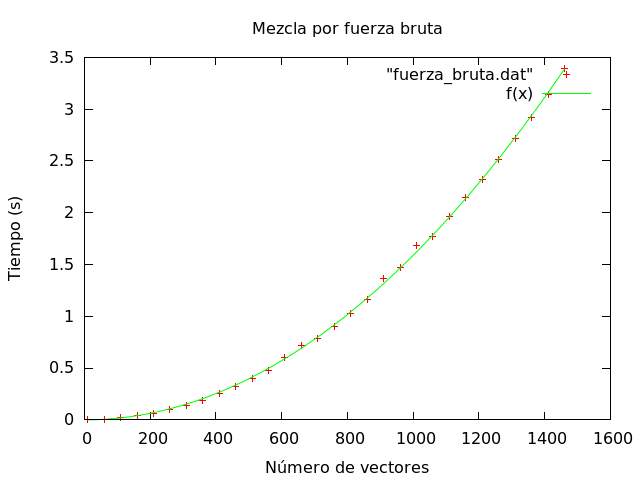
\includegraphics[width=0.6\textwidth]{../Obligatorio/Graficas/fuerza_bruta_kvectores.png}
	\caption{Fuerza bruta con 200 elementos cada vector} 
	\label{fig:f_kvectores} 
\end{figure}

\newpage
%%%%%%%%%%%%%%%%%%%%%%%%%%%%%%%%%%%%%%%%%%%%%
Para la parte en la que cambiamos el n\'umero de elementos ajustamos la funci\'on 
$f(x) = ax$ ya 	que en $T(k, n) = nklog_2k, \ klog_2k$ es una constante, concretamente $200$.

\begin{center}
\fcolorbox{gray75}{gray97}{
$a               = 0.00031202$}
\fcolorbox{gray75}{gray97}{
Correlation:  $r = 0.9934$}
\end{center}

Para obtener una funci\'on ajustada del tipo $g(x)=c\cdot knlog_2k$, calculamos $c=\frac{a}{100\cdot log_2(100)}, c \in \mathbb{R}$,

\begin{figure}[htb] 
\centering
	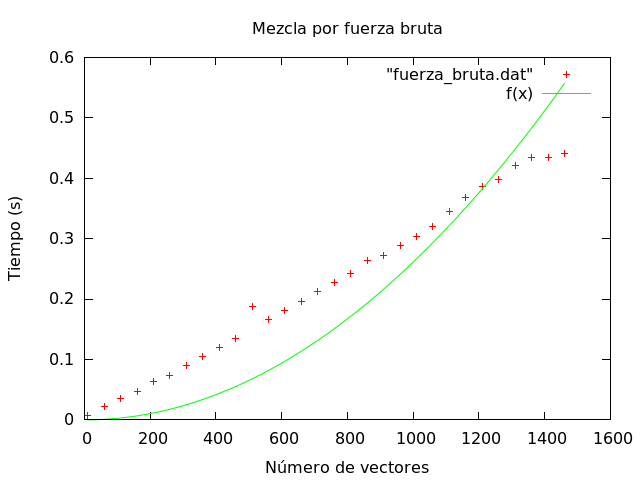
\includegraphics[width=0.6\textwidth]{../Obligatorio/Graficas/fuerza_bruta_nelementos.png}
	\caption{Fuerza bruta con 200 vectores} 
	\label{fig:f_nelementos} 
\end{figure}
\newpage


\subsubsection{Mezcla con divide y vencer\'as}
La funci\'on ajustada ha sido $f(x) = ax(log(x)/log(2))$

\begin{center}
\fcolorbox{gray75}{gray97}{
$a               = 4.52594\cdot 10^{-6}$}
\fcolorbox{gray75}{gray97}{
Correlation:  $r = 0.9863$}
\end{center}

\begin{figure}[htb] 
\centering
	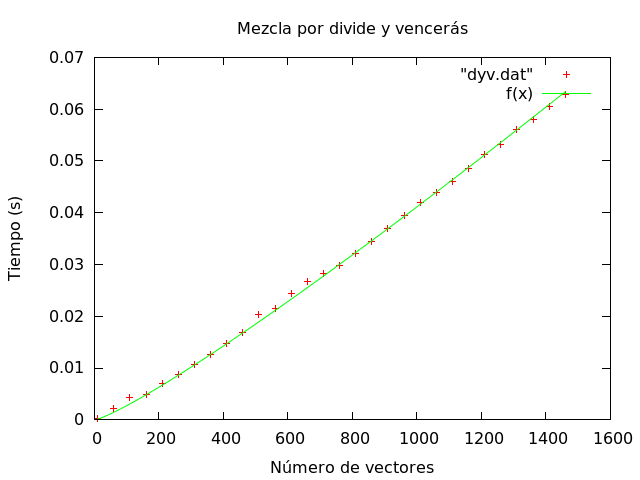
\includegraphics[width=0.6\textwidth]{../Obligatorio/Graficas/dyv_kvectores.png}
	\caption{Divide y vencerás con 200 elementos cada vector} 
	\label{fig:d_kvectores} 
\end{figure}

%%%%%%%%%%%%%%%%%%%%%%%%%%%%%%%%%%%%%%%%%%%%%%%%%%%%%%%%%%
Si ahora fijamos $k=200$ y hacemos variable el n\'umero de elementos debemos ajustar la funci\'on $f(x) = ax(log(x)/log(2))$

\begin{center}
\fcolorbox{gray75}{gray97}{
$a               = 3.03036\cdot 10^{-6}$}
\fcolorbox{gray75}{gray97}{
Correlation:  $r = 0.9933$}
\end{center}

\begin{figure}[htb] 
\centering
	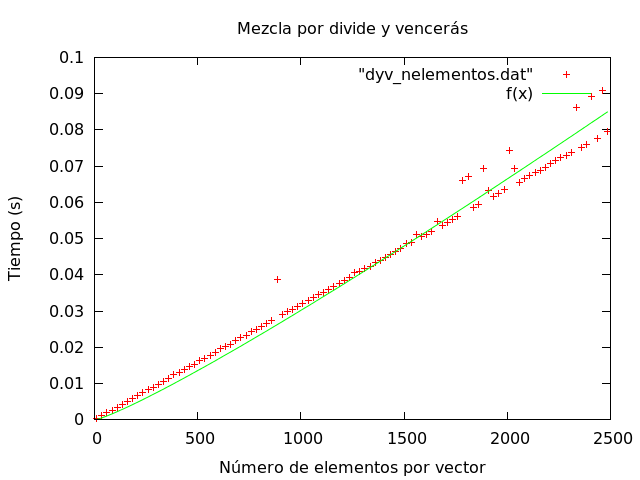
\includegraphics[width=0.6\textwidth]{../Obligatorio/Graficas/dyv_nelementos.png}
	\caption{Divide y venceras con 200 vectores} 
	\label{fig:d_nelementos} 
\end{figure}
\newpage

%%%%%%%%%%%%%%%%%%%%%%%%%%%%%%%%%%%%%%%%%%%%%%%%
\subsubsection{Comparativa}
Como podemos deducir del estudio te\'orico, las diferencias entre fuerza bruta y divide y vencer\'as se aprecian algo m\'as al variar los vectores.
\begin{figure}[htb] 
\centering
	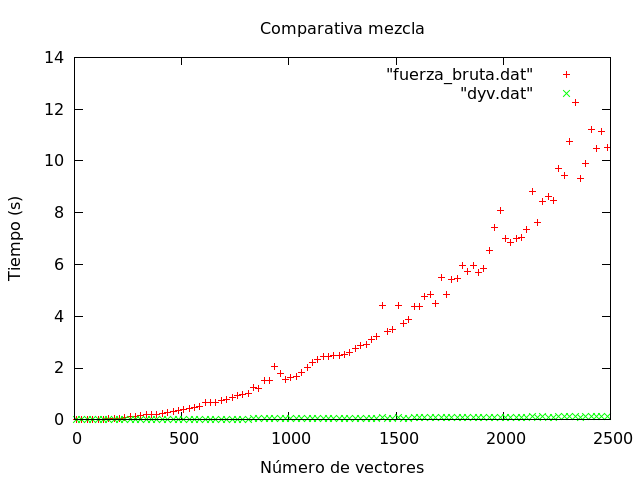
\includegraphics[width=0.6\textwidth]{../Obligatorio/Graficas/comparativa_kvectores.png}
	\caption{Comparativa con 200 elementos cada vector} 
	\label{fig:comp_kvectores} 
\end{figure}

\begin{figure}[htb] 
\centering
	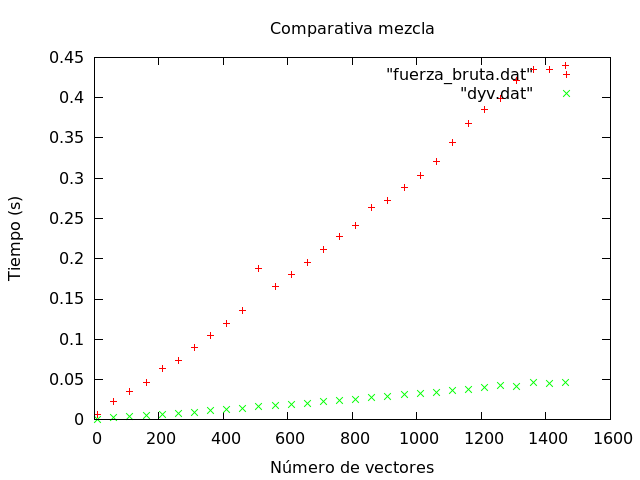
\includegraphics[width=0.6\textwidth]{../Obligatorio/Graficas/comparativa_nelementos.png}
	\caption{Comparativa con 200 vectores} 
	\label{fig:comp_nelementos} 
\end{figure}

\newpage
Si queremos combinar los resultados podemos variar simult\'aneamente el n\'umero de vectores y los elementos del vector tenemos que crear gr\'aficas en $3$ dimensiones.
De esta forma podemos comprobar que el n\'umero de vectores es un factor m\'as influyente que el n\'umero de elementos de cada vector. Sin embargo este es un dato que se aprecia en el algoritmo por fuerza bruta, en el divide y vencer\'as apenas se nota diferencia.

\begin{figure}[htb] 
\centering
	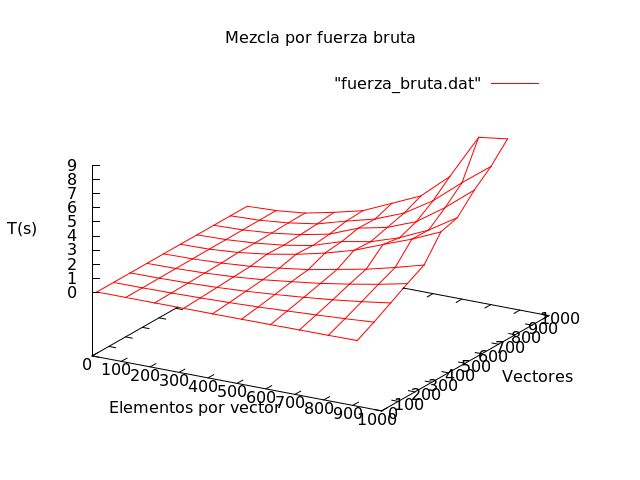
\includegraphics[width=0.6\textwidth]{../Obligatorio/Graficas/3d_fuerza_bruta.png}
	\caption{3d fuerza bruta} 
	\label{fig:3d_f} 
\end{figure}

\begin{figure}[htb] 
\centering
	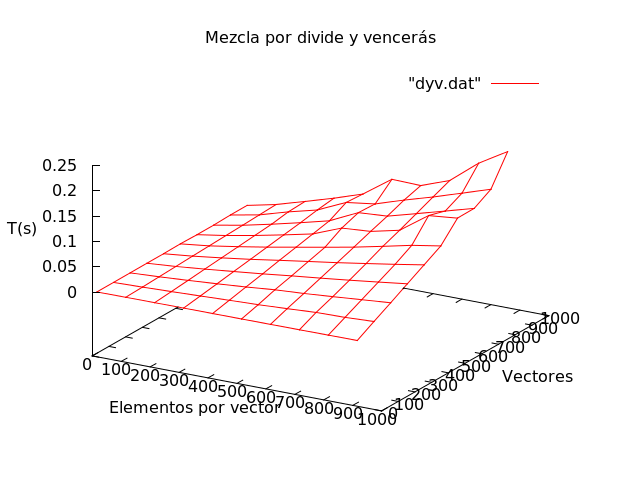
\includegraphics[width=0.6\textwidth]{../Obligatorio/Graficas/3d_dyv.png}
	\caption{3d divide y vencerás} 
	\label{fig:3d_d} 
\end{figure}

\newpage

{\ }

\newpage


